% !TEX root=foo.tex
\section{Findings}
\label{sec:findings}

\subsection{Qualitative Coding}

As discussed in the previous section, we filtered 516 comments based on the initial binary coding which account for more than half (51.6\%) of the dataset of 1000 comments. Later, we performed second level thematic coding based on 8 themes (although we report 7, the clarification on eighth one is given in Methods section) mentioned previously to see what is the underlying factor for either social media \textit{Non-use} or user dissatisfaction. The findings are summarized in Table~\ref{table:coding category}.


\begin{table*}[t!]

\centering
\begin{tabular}{p{0.20\linewidth}|p{0.2\linewidth}|p{0.1\linewidth}|p{0.4\linewidth}}
\hline
{Theme} & {Example Topic} & {\# Comments} & {Example Comment}  \\
\hline
Facebook Functionality  & advertisement, news feed, messenger, tagging   & 245(222) & \textit{"After all, Facebook users have NO CHOICE but to use Facebook and allow them to force you to watch ads. Really, you have no choice, none at all. Suck it up and get used to it."}\\\hline

Privacy and Security & selling data, stalking, apps accessing mobile data & 168(158) &\textit{"Facebook is essentially saying you don't HAVE to enter into an agreement with them in order for them to keep track of you."}\\\hline

Personal Preferences & waste of time, do not like using Facebook, do not care & 96(85) &\textit{"who cares? I DO NOT GIVE A DAMN, I don't use Facebook or linkedin, and my computer blocks resolving those domains."}\\\hline

Negative Perceptions of Facebook & creepy, blocked Facebook, hate words & 76(64) &\textit{"Seriously, I've distrusted Facebook from the very start, and never will trust it. Given that Zuckerberg is on record as saying that anyone who trusts him is a fool, I'm going to work accordingly. I've got better things to do with my life then spend it tethered to bullshit."}\\\hline

Audience & sharing data with friends, audience changing, impression management & 67(63) &\textit{"The proper form that the apology should have taken is this, "I am sorry that anyone was offended because someone added me to a Facebook Group that included tasteless comments, comments that may constitute illegal threats of violence, made by someone else. I do not condone such language."}\\\hline

Influence of External Factors & forced to use, job, politics & 58(45) &\textit{"About a year ago, keeping up with FB started to seem like a bit of a job, ain't nobody paying me to do it, and it has seldom if ever proved all that helpful or useful in ways that couldn't be accomplished via other, less intrusive, less annoying ways"}\\\hline

Non-Facebook Media Use & migrating to other social media, preferring other social media, telephone & 27(21) &\textit{"My teenage daughters, and all their friends, live and breathe SnapChat. Not one of them is on Facebook. This could change, but I don't anticipate any of them switching."}\\\hline
\hline
\end{tabular}
\caption{Themes from second level thematic coding, example topic, number of comments, and one representative example. Within parentheses is the number of comments where both rater agreed for that theme and outside where either one agreed.}
    \label{table:coding category}
\end{table*}


The distribution of the comments falling into each theme is depicted in Figure~\ref{fig:figure1}. We have shown, for each theme, the number of comments that fell into that theme. It is obvious from the graph that in all cases the raters disagreed to some extent. The percentages shown as label on blue bars does not sum to 100 since one comment could be associated with multiple themes therefore those comments are counted multiple times.

\begin{figure}
  \centering
  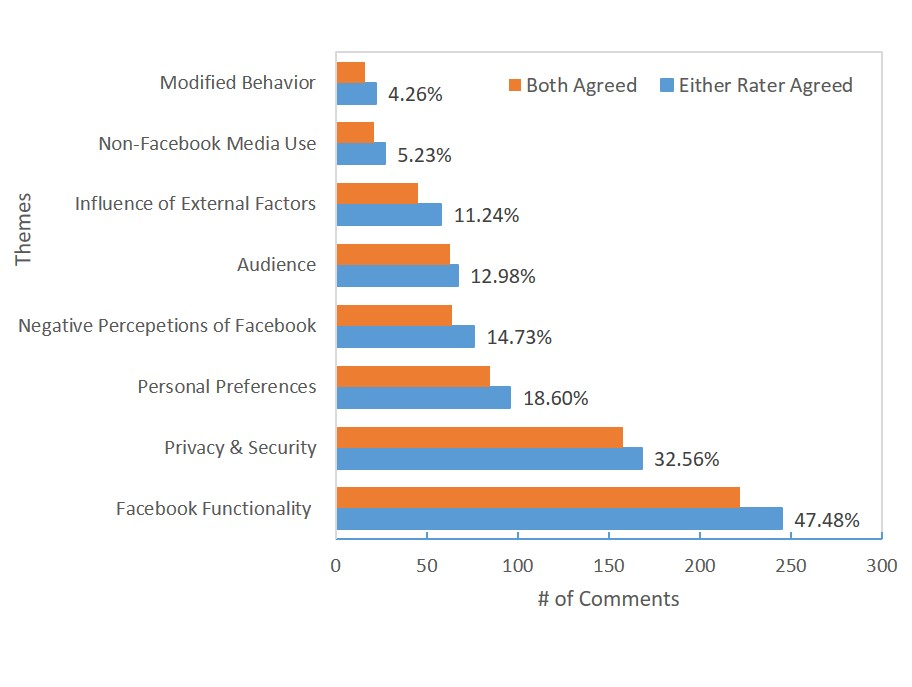
\includegraphics[width=1.0\columnwidth]{figures/fig7.jpg}
  \caption{Distribution of 516 \emph{Non-use} comments into themes.}~\label{fig:figure1}
\end{figure}

\subsection{Natural Language Processing}

\subsubsection{Wordcloud}
We performed multiple NLP based analysis on our dataset to gain deeper understanding. The initial unigram wordcloud that was made on overall 516 \textit{Non-use} related comments (regardless of theme) is shown in Figure~\ref{fig:figure2}(a). Drawing a bigram (Figure~\ref{fig:figure2}(b)) and trigram (Figure~\ref{fig:figure2}(c)) helped us surface further innate emotions and reasoning of Facebook haters.


% \begin{figure*}[t]
% \centering
% \subfloat[Unigram wordcloud ]{
%   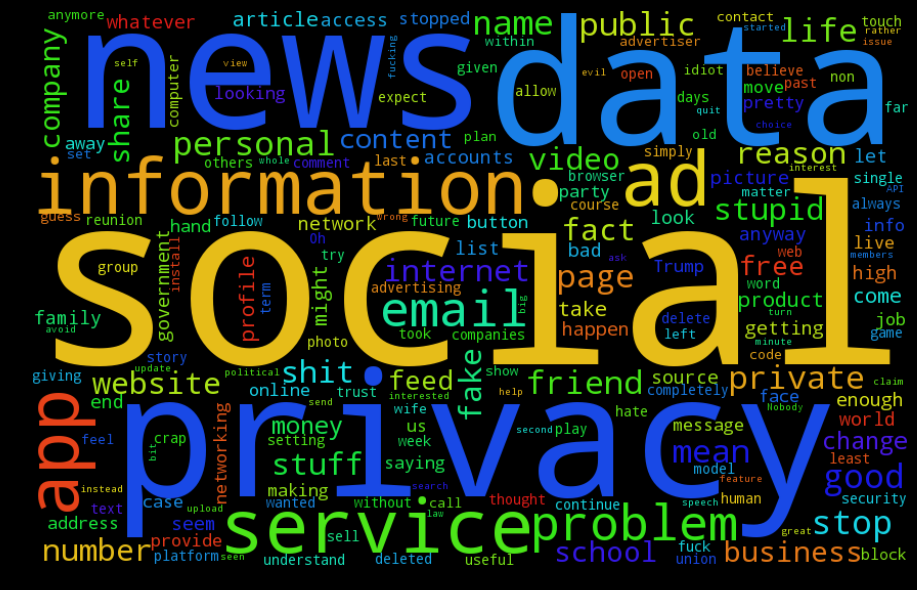
\includegraphics[width=60mm, height=4cm]{figures/fig2.png}
% }\hfill
% \subfloat[Bigram wordcloud]{
%   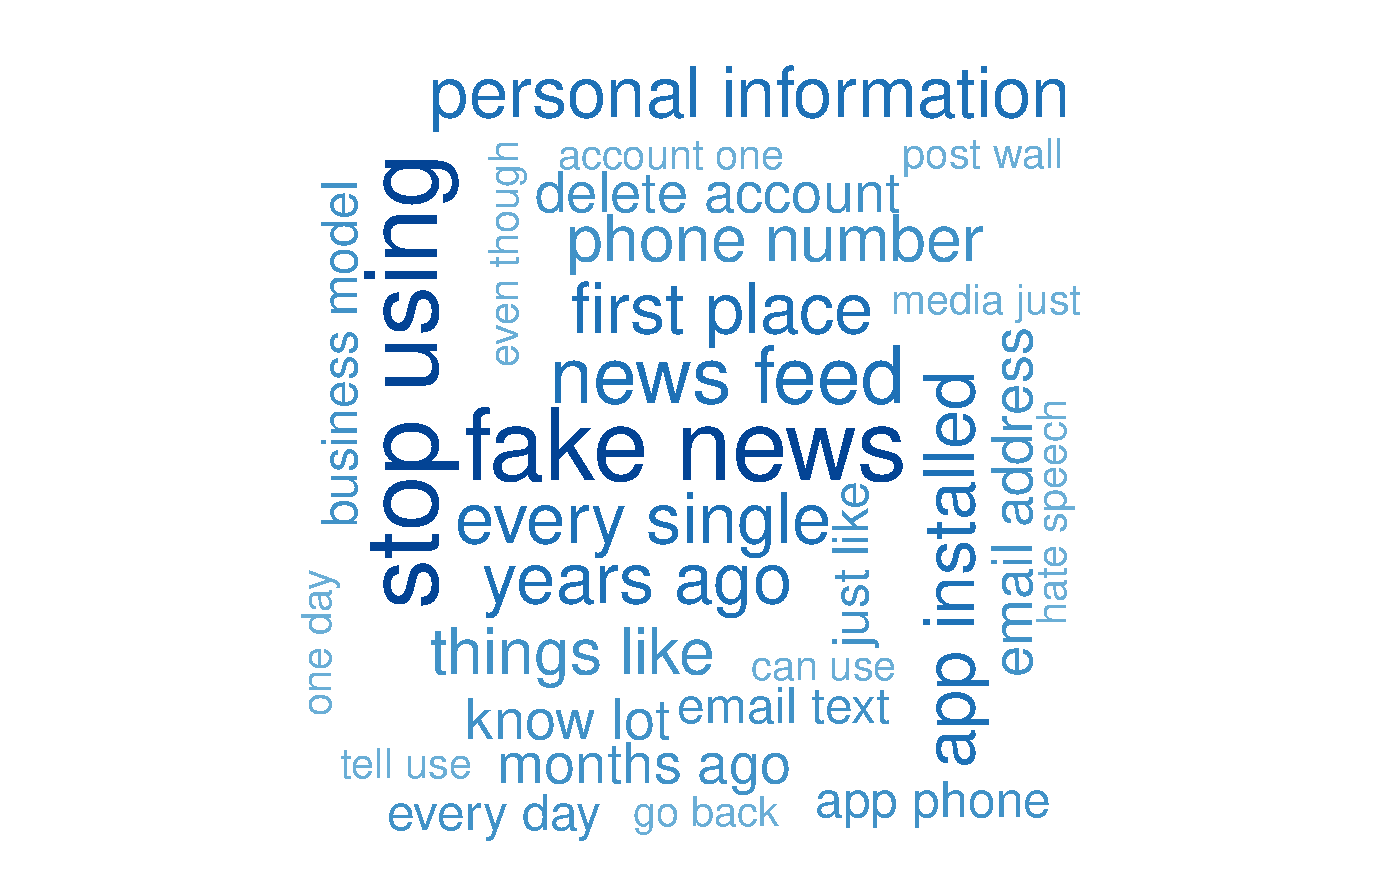
\includegraphics[width=90mm]{figures/fig3.eps}
% }\hfill

% \subfloat[Trigram wordcloud]{
%   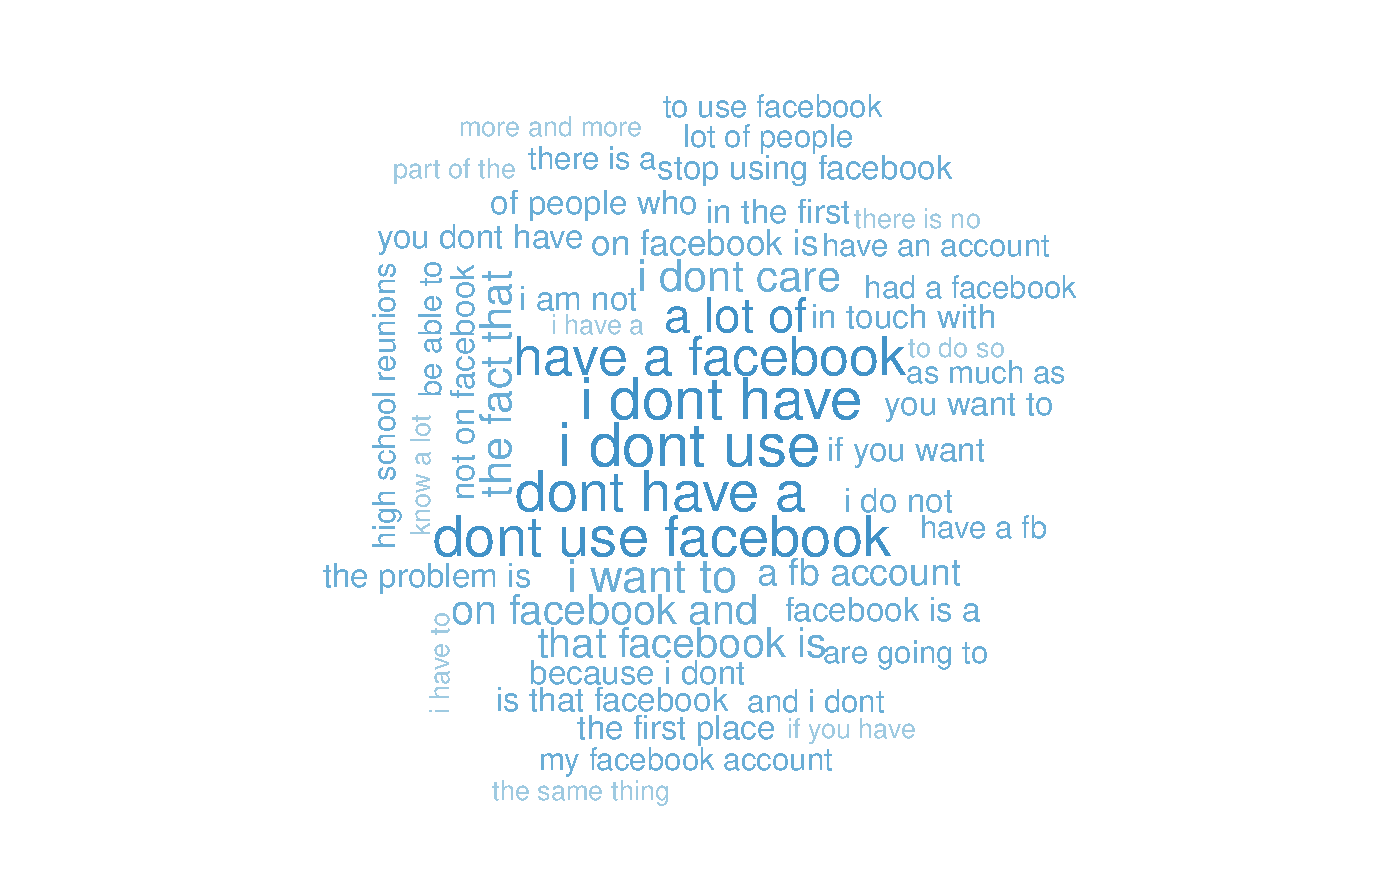
\includegraphics[width=90mm]{figures/fig4.eps}
% }
% \caption{Visualization of 516 \textit{Non-use} comments.}~\label{fig:figure2}
% \end{figure*}


\begin{figure*}
\subfloat[Unigram wordcloud\label{fig:test1}]
  {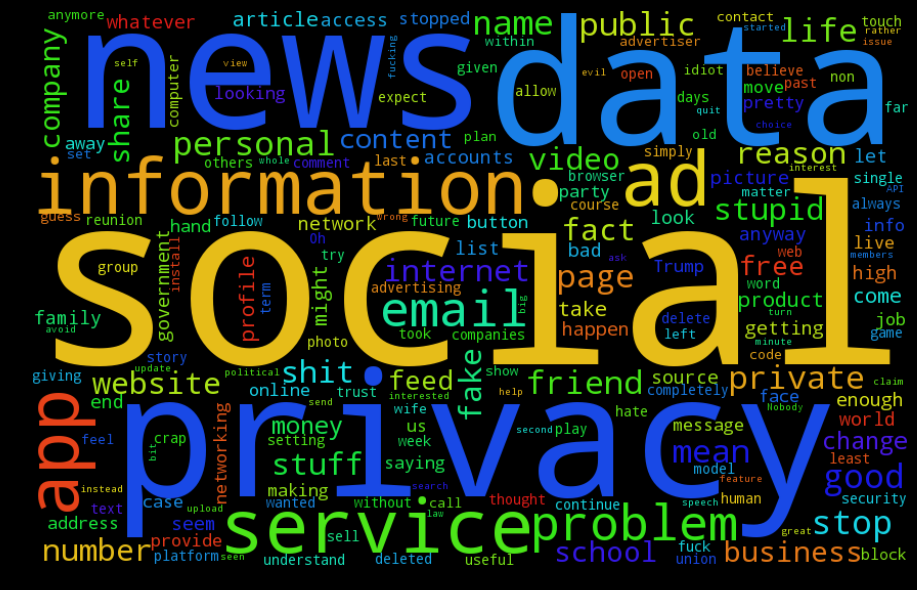
\includegraphics[width=.3\linewidth, height=4cm]{figures/fig2.png}}\hfill
\subfloat[Bigram wordcloud\label{fig:test2}]
  {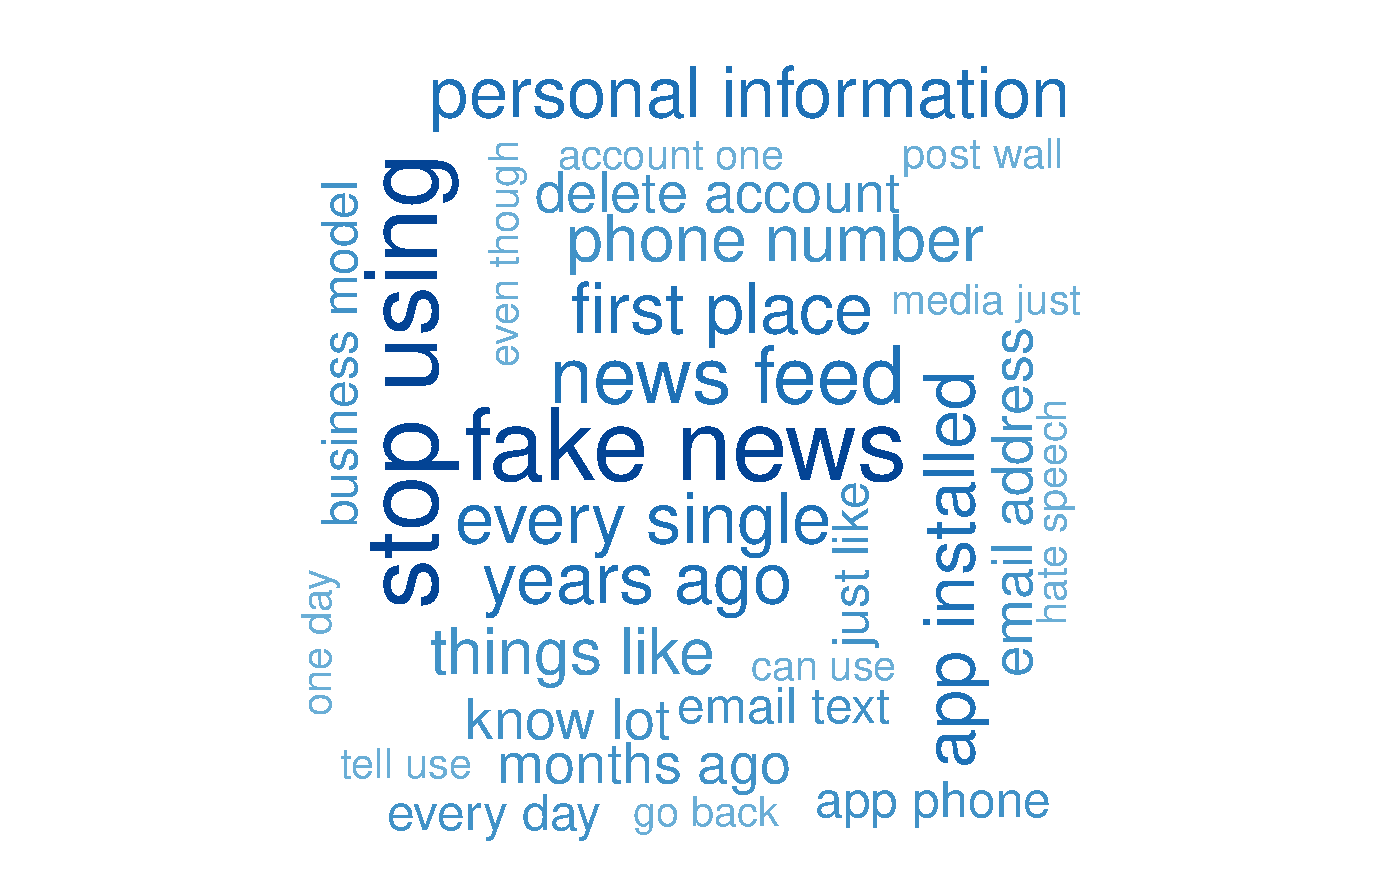
\includegraphics[width=.35\linewidth, height=4cm]{figures/fig3.eps}}\hfill
\subfloat[Trigram wordcloud\label{fig:test3}]
  {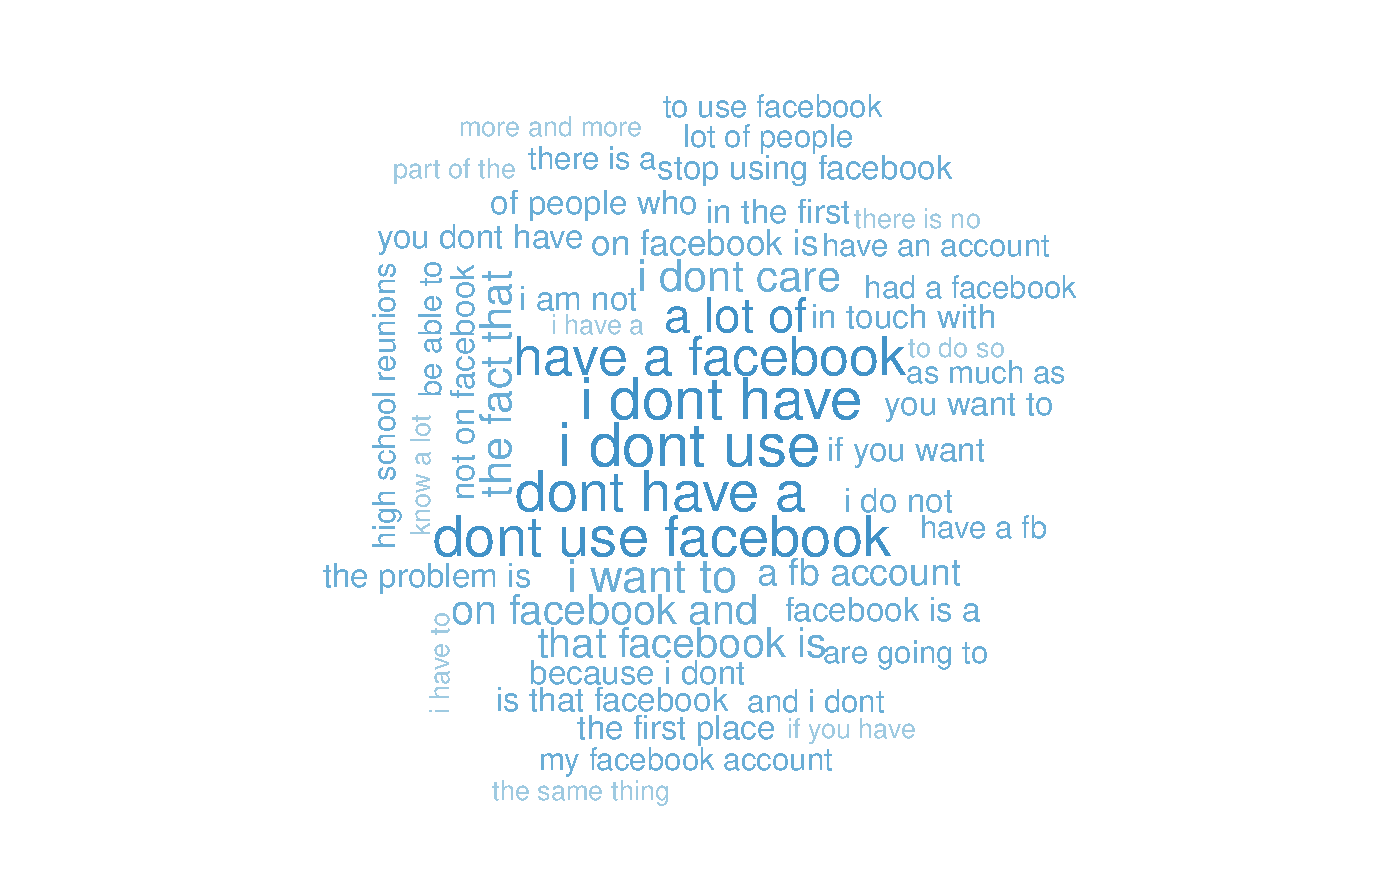
\includegraphics[width=.35\linewidth, height=4cm]{figures/fig4.eps}}
\caption{Visualization of 516 \textit{Non-use} comments.}~\label{fig:figure2}
\end{figure*}




\subsubsection{Topic Modeling}

Our trained LDA model produced 8 topics. Each topic is associated with a weight-distributed set of words. For each weight $w_i$, the weights are normalized such that, $\sum_{i=1}^n w_i=1$. Table ~\ref{tab:table3} lists each topic associated with the word distribution and few selected highly representative words from that distribution those the authors found a match while coding the comments.


\begin{table*}[ht]

\centering
\begin{tabular}{p{0.1\linewidth}|p{0.70\linewidth}|p{0.15\linewidth}}
\hline
\head{Topic \#} & \head{Word Distribution} & \head{Representative Words}\\
\hline
1       & 0.008*"app" + 0.005*"company" + 0.004*"reason"+ 0.004*"feed" + 0.004*"speech" + 0.004*"apps" + 0.004*"data" + 0.004*"privacy" + 0.004*"hate" + 0.004*"always" & hate,privacy\\\hline
2 & 0.012*"social" + 0.008*"stop" + 0.007*"news" + 0.006*"privacy" + 0.006*"ads" + 0.005*"device" + 0.005*"friend" + 0.004*"block" + 0.004*"seen" + 0.004*"political" & news,ads,block\\\hline

3 & 0.011*"social" + 0.009*"information" + 0.007*"stuff" + 0.006*"data" + 0.004*"mean" + 0.004*"provide" + 0.004*"source" + 0.004*"private" + 0.004*"government" + 0.004*"looking" & data,private\\\hline

4 & 0.010*"privacy" + 0.007*"email" + 0.006*"private" + 0.006*"service" + 0.006*"ads" + 0.005*"social" + 0.005*"profile" + 0.004*"information" + 0.004*"world" + 0.004*"name" & privacy,information\\\hline

5 & 0.008*"privacy" + 0.007*"union" + 0.007*"social" + 0.005*"data" + 0.005*"stopped" + 0.005*"personal" + 0.004*"access" + 0.004*"code" + 0.004*"dropped" + 0.004*"left" & stopped,left,dropped \\\hline

6 & 0.013*"information" + 0.010*"social" + 0.009*"personal" + 0.007*"data" + 0.004*"play" + 0.004*"upload" + 0.004*"online" + 0.004*"number" + 0.004*"take" + 0.004*"face"  & social,personal\\\hline

7 & 0.011*"news" + 0.006*"deleted" + 0.005*"tag" + 0.005*"information" + 0.005*"articles" + 0.004*"fake" + 0.004*"business" + 0.004*"stop" + 0.004*"privacy" + 0.004*"free" & deleted,fake,stop\\\hline

8 & 0.008*"social" + 0.007*"data" + 0.007*"news" + 0.005*"money" + 0.005*"might" + 0.004*"problem" + 0.004*"us" + 0.004*"making" + 0.004*"information" + 0.004*"last"  & money,problem\\
\hline
\end{tabular}
\caption{LDA topic modeling on the dataset.}
    \label{tab:table3}
\end{table*}

To confirm the results obtained from LDA model, the topics found from Non-negative Matrix Factorization (NMF) were compared. Table ~\ref{tab:table4} summarizes the top 5 topic words of each topic (Highlighted are the most intereseting and relevant topic words.)


\newcommand{\head}[1]{\textnormal{\textbf{#1}}}

\begin{table}[!ht]
% let LaTeX figure out optimal amount of intercolumn whitespace:
\setlength\tabcolsep{0pt} 

\begin{tabular*}{\columnwidth}{@{\extracolsep{\fill}}c*{3}{T{1.8}}cT{1.8}}  
\toprule
\head{Topic \#} & \head{Topic Words} \\
\midrule
\textbf{1}              & \textbf{social} networking network face email &    \\                    
   \textbf{2} & \textbf{news} \textbf{fake} feed articles trump & \\
   \textbf{3} & \textbf{friend} \textbf{info} word profile mean & \\
   \textbf{4} & \textbf{privacy} information \textbf{private} \textbf{personal} public & \\
   \textbf{5} & \textbf{data} business personal good fact & \\
   \textbf{6} & app installed \textbf{ads} guess android & \\
   \textbf{7} & accounts \textbf{stopped} \textbf{hell} play platform  & \\
   \textbf{8} & \textbf{shit} \textbf{hate} \textbf{share} service public & \\
  \hline
\bottomrule 
\end{tabular*}
\caption{NMF topic modeling on the dataset.}
    \label{tab:table4}
\end{table}

\subsubsection{Sentiment Analysis}

Initially we performed sentiment analysis with VADER tool on our overall set of 516 \textit{Non-use} comments. Then we looked into each of the eight themes to see how the user sentiment compares according to comments belonging to each theme. The VADER tool returns four different measures of sentiment: \textit{pos}, \textit{neg}, \textit{neu} and \textit{compund score}. The compound score can be found by summing the valence scores of each word in the lexicon, adjusted according to the rules. Then it is normalized between -1 to 1, where -1 being extreme negative and +1 being extreme positive. Typically the threshold adopted by researchers ~\cite{hutto2014vader} is: \textit{compound score} >= 0.5 is positive; \textit{compound score} <=-0.5 is negative and anything between -0.5 and 0.5 is neutral. Values of \textit{pos}, \textit{neg} and \textit{neu} can be used instead if multidimensional sentiment analysis of a sentence is desired, where they indicate the percentage of the text that fell into those sentiment categories. In Figure ~\ref{fig:figure6}, we show the box plots of compound sentiment scores for 8 themes as well as the overall set of comments side by side.  


\begin{figure}[t!]
  \centering
  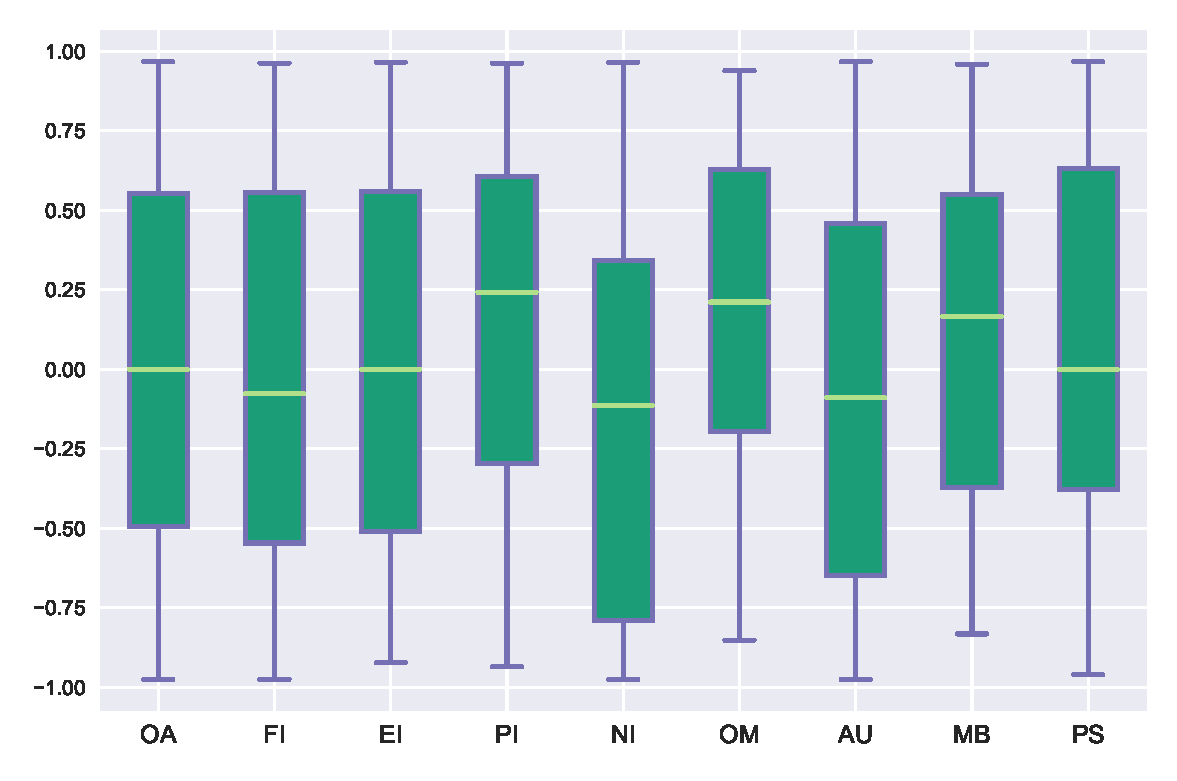
\includegraphics[width=1.0\columnwidth]{figures/fig6.eps}
  \caption{Box plots of compound sentiment scores of each theme using VADER tool. (OA = Overall, FI = Facebook Functionality, EI= Influence of External Factors, PI = Personal Preferences, NI = Negative Perceptions of Facebook, OM = Non-Facebook Media Use, AU = Audience, MB = Modified Behavior, PS = Privacy \& Security)}~\label{fig:figure6}
\end{figure}

For our analysis, we categorize the sentiment associate with the compound score as: $compound score >= 0.5$ is extremely positive; $compound score <-0.5$ is extremely negative, $ 0<=compound score<0.5$ is positive and $-0.5<=compound score<0$ is negative. We calculate the percentage negative per theme as: $$\frac{\text{number of extreme negatives + number of negatives}}{\text{total number of comments belonging to that theme}}$$

The results are reported in Table ~\ref{tab:table5}.

% \newcommand{\head}[1]{\textnormal{\textbf{#1}}}

% \begin{table}[!ht]
% % let LaTeX figure out optimal amount of intercolumn whitespace:
% \setlength\tabcolsep{0pt} 

% \begin{tabular*}{\columnwidth}{@{\extracolsep{\fill}}c*{3}{T{1.8}}cT{1.8}}  
% \toprule
% \head{Theme} & \head{\# Extreme Pos} & \head{\# Pos} & \head{\# Extreme Neg} & \head{\# Neg} & \head{\% Neg}\\
% \midrule
% \textbf{FI}              & 66     & 53 & 59 & 67 & 51.42\%\\                    
%   \textbf{EI} & 16      & 17 & 9 & 16 & 43.10\% \\
%   \textbf{PI} & 33      & 29 & 23 & 11 & 35.41\%\\
%   \textbf{OM} & 10      & 8 & 5 & 4 & 33.33\%\\
%   \textbf{NI} & 13      & 21 & 11 & 31 & 55.26\%\\
%   \textbf{AU} & 17      & 14 & 16 & 20 & 53.73\%\\
%   \textbf{PS} & 58      & 38 & 39 & 33 & 42.85\%\\
%   \textbf{MB} & 8      & 4 & 7 & 3 & 45.45\%\\
%   \hline
% \bottomrule 
% \end{tabular*}
% \caption{Sentiment distribution for 8 themes using VADER method. (FI = Facebook Functionality, EI= Influence of External Factors, PI = Personal Preferences, NI = Negative Perceptions of Facebook, OM = Non-Facebook Media Use, AU = Audience, MB = Modified Behavior, PS = Privacy \& Security)}
%     \label{tab:table5}
% \end{table}


\begin{table}[t!]

\centering
\begin{tabular}{p{0.1\linewidth}|p{0.18\linewidth}|p{0.1\linewidth}|p{0.18\linewidth}|p{0.1\linewidth}|p{0.1\linewidth}}
\hline
\head{Theme} & \head{\# Extreme Pos.} & \head{\# Pos.} & \head{\# Extreme Neg.} & \head{\# Neg.} & \head{\% Neg.}\\
\midrule
\textbf{OA}              & 140     & 135 & 127 & 113 & 46.51\%\\
\textbf{FI}              & 66     & 53 & 67 & 59 & 51.42\%\\                    
  \textbf{EI} & 16      & 17 & 16 & 9 & 43.10\% \\
  \textbf{PI} & 33      & 29 & 11 & 23 & 35.41\%\\
  \textbf{OM} & 10      & 8 & 4 & 5 & 33.33\%\\
  \textbf{NI} & 13      & 21 & 31 & 11 & 55.26\%\\
  \textbf{AU} & 17      & 14 & 20 & 16 & 53.73\%\\
  \textbf{PS} & 58      & 38 & 33 & 39 & 42.85\%\\
  \textbf{MB} & 8      & 4 & 3 & 5 & 45.45\%\\
  \hline
\bottomrule 
\end{tabular}
\caption{Sentiment distribution for 8 themes using VADER method. (OA = Overall, FI = Facebook Functionality, EI = Influence of External Factors, PI = Personal Preferences, NI = Negative Perceptions of Facebook, OM = Non-Facebook Media Use, AU = Audience, MB = Modified Behavior, PS = Privacy \& Security)}
    \label{tab:table5}
\end{table}

% Finally, our trained logistic regression model that was trained on Kaggle data\footnote{\url{https://inclass.kaggle.com/c/si650winter11}} achieved precision, recall and f1-score of 0.98, 0.98 and 0.98 respectively. When applied on unseen comments from our dataset, the classifier results are reported in Table ~\ref{tab:table5}

% \newcommand{\head}[1]{\textnormal{\textbf{#1}}}

% \begin{table}[!ht]
% % let LaTeX figure out optimal amount of intercolumn whitespace:
% \setlength\tabcolsep{0pt} 

% \begin{tabular*}{\columnwidth}{@{\extracolsep{\fill}}c*{3}{T{1.8}}cT{1.8}}  
% \toprule
% \head{Theme} & \head{\#Pos} & \head{\#Neg} & \head{\% Neg}\\
% \midrule
% \textbf{Facebook Functionality}              & 80     & 165 & 67.34\\                    
%   \textbf{Influence of External Factors} & 29      & 29 & 50.00\\
%   \textbf{Personal Preferences} & 25      & 71 & 73.95\\
%   \textbf{Negative Perceptions of Facebook} & 24      & 52 & 68.4\\
%   \textbf{Non-Facebook Media Use} & 4      & 23 & 85.18\\
%   \textbf{Audience} & 20      & 47 & 70.14\\
%   \textbf{Modified Behavior} & 7      & 15 & 68.18\\
%   \textbf{Privacy \& Security} & 62      & 106 & 63.09\\
%   \hline
% \bottomrule 
% \end{tabular*}
% \caption{Sentiment distribution for 8 themes using Logistic Regression method.}
%     \label{tab:table5}
% \end{table}

